\documentclass[11pt,a4paper]{report}
\usepackage{fullpage}
\usepackage[polish]{babel}
\usepackage{polski}
\usepackage[utf8]{inputenc}
\usepackage[T1]{fontenc}
\usepackage{indentfirst}
\usepackage{type1ec}
\usepackage{amsthm}
\usepackage{amsfonts}
\usepackage{listings}
\headsep = 30pt
%\linespread{2}



\selectlanguage{polish}
\frenchspacing

\title{\textbf{Wpływ wykorzystania archiwum do mutacji różnicowej w algorytmie ewolucji różnicowej na jakość optymalizacji w przestrzeni ciągłej.}}
\author{Andrzej Fiedukowicz}
\date{}

\usepackage{mathtools}
\usepackage{fancyhdr}
\pagestyle{fancy}

\fancyhead{}
\fancyhead[R]{\thepage}
\renewcommand{\chaptermark}[1]{\markboth{\chaptername\ \thechapter.\ #1}{}}
\fancyhead[L]{\leftmark}
\fancyfoot{}
\renewcommand{\headrulewidth}{0.4pt}

\fancyheadoffset[]{0pt}

\fancypagestyle{plain}{
\fancyhf{}
\fancyfoot[C]{\bfseries \thepage}
\renewcommand{\headrulewidth}{0pt}
\renewcommand{\footrulewidth}{0pt}}

\begin{document}
\DeclareGraphicsExtensions{.pdf,.png,.jpg}

\maketitle
\tableofcontents

\newpage
\subsubsection{Streszczenie}
\par{
\emph{
Algorytmy ewolucji różnicowej (DE) występują w wielu wariantach i odmianach, których właściwości są cały czas badane. Jedną z proponowanych modyfikacji tego algorytmu stanowi wykorzystanie przy operatorze mutacji różnicowej osobników pochodzących z szerszego niż jednopokoleniowego okna historii [MS:PrzydaloBySięŹródło, jeśli nie -- zmiana sformułowania].
}
}
\par{
\emph{
Niniejsza praca opisuje proces opracowywania metody zastosowania archiwum osobników w celu poprawy jakości wyników uzyskiwanych w ewolucji różnicowej. W dalszej części praca skupia się na sprawdzeniu hipotezy o możliwości poprawy klasycznego schematu ewolucji różnicowej DE/rand/1/bin przez wykorzystanie archiwum.
Badania skuteczności poszczególnych metod opracowane są w oparciu o zestaw funkcji testowych opracowanych w ramach konferencji IEEE Congress on Evolutionary Computation 2013 (CEC2013) [MS:Potrzebne Źródło].
}
}
\par{
\emph{
Niniejsza praca odnosi się także do możliwości i skuteczności wykorzystania w procesie ewolucji różnicowej punktu środkowego populacji, badając jego wartość w czasie działania wszystkich testowanych wariantów algorymtów.
}
}
\subsubsection{Słowa kluczowe}
\par{
\emph{Ewolucja Różnicowa, DE, Algorytmy Ewolucyjne, AE, Optymalizacja, Optymalizacja black0--box}
}
\subsubsection{Abstract}
\par{
\emph{There are many forms of differential evolution algorithms (DE), which properties are yet to be discovered. One of possible modifications of those algorithms is using historical points to perform differential mutation. [MS:PrzydałoBySięŹródło]}.
}
\par{
\emph{
This thesis describes development process of method of using such archive to increase DE results quality. Hereafter this thesis is checking hipotesis about possibility of improving classic DE/rand/1/bin by using archive. All experiments performed during this reasearch are based on benchmark functions set developed during the IEEE Congress of Evolutionary Computation 2013 conference (CEC2013) [MS:Potrzebne Źródło].
}
}
\par{
\emph{
This thesis also refers to a possiblity and effectiveness of using middle point of population to improve quality of DE results by checking its value in all tested variants of DE. 
}
}
\subsubsection{Keywords}
\par{
\emph{Differential Evolution, DE, Evolutionary Algorithms, EA, Optimialization, Black--box optimalization}
}

\chapter{Wstęp}
\par{
Problem optymalizacji jest jednym z najczęściej pojawiających się w praktycznych zastosowaniach problemów numerycznych. Sama powszechność podstawowego problemu, ale także możliwość sprowadzenia do problemu optymalizacji problemów klasyfikacji, regresji, grupowania czy też określając szerzej -- uczenia maszynowego \cite{SearchingInteligent,SpringerIntroToEvol}, sprawia, że przed algorytmami optymalizacji stawiane są coraz bardziej złożone i wymagające zadania.
}
\par{
Stale zwiększający się poziom trudności problemów optymalizacyjnych jak i ciągła niedoskonałość dotychczas wytworzonych metod ich rozwiązywania powoduje duże zainteresowanie badaniami dotyczącymi tworzenia coraz doskonalszych, szybszych i dających lepsze rezultaty algorytmów owe problemy rozwiązujących \cite{StateOfArt}.
}

\section{Definicja problemu}
\par{
Praca ta, umiejsciowiona została w kontekście rozwiązywania problemów optymalizacji gdzie analityczne wyznaczenie ekstremum funkcji jest niemożliwe bądź w ogóle nie jest znana jej analityczna forma. Zakłada się bowiem, że zadanie jest zdefiniowane następująco \cite{StrojnowskiOptymalizacja2}:
}
\newtheorem{OptDefinition}{Definition}
\par{
\begin{OptDefinition}
Problem globalnej optymalizacji funkcji $f: X \rightarrow \mathbb{R}$ polega na wyznaczeniu takiego $x_0 \in X$, że:
\begin{center}
	$\forall_{x \in X} f(x_0) \leq f(x)$
\end{center}
\end{OptDefinition}
\par{
Dla celów tej pracy przyjmuje się możliwość zbadania wartości funkcji $f$ w dowolnym punkcie ze zbioru $X$, jednak brak możliwości bezpośredniego zbadania jakichkolwiek innych własności tejże funkcji. W tej formie problem ten można nazwać problemem optymalizacji funkcji zadanej w formie reaktywnej (\emph{Black--box optimization}).
}
\par{
W ramach rozpatrywanych problemów istnieje także możliwość, że dziedzina funkcji $f$ jest szersza niż zbiór rozwiązań dopuszczalnych. W takich wypadkach mówimy o problemie optymalizacji z ograniczeniami.
\begin{OptDefinition}
Problem globalnej optymalizacji funkcji $f: X \rightarrow \mathbb{R}$ z ograniczeni $X_D \subset X$ polega na wyznaczeniu takiego $x_0 \in X_D$, że:
\begin{center}
	$\forall_{x \in X_D} f(x_0) \leq f(x)$
\end{center}
\end{OptDefinition}
Dla tego rodzaju problemów, możliwe jest wyznaczanie wartości funkcji w całej jej dziedzinie $X$, jednak poszukiwane rozwiązanie musi pochodzić z ograniczonego zbioru $X_D$.
Problem globalnej optymalizacji funkcji z ogarniczeniami stanowi uogólnienie problemu optymalizacji globalnej bez ogarniczeń.
}
\par{
Szczególnym przypadkiem problemu optymalizacji globalnej z ogarniczeniami jest przeszukiwanie przestrzeni ciągłej. 
\begin{OptDefinition}
Problem globalnej optymalizacji funkcji $f: \mathbb{R}^n \rightarrow \mathbb{R}$ z ograniczeniem $X_D = \{x \in \mathbb{R}^n: g_1(x) \leq 0, g_2(x) \leq 0, \ldots, g_m(x) \leq 0\}$ nazywamy problemem optymalizacji globalnej przestrzeni ciągłej z ogarniczeniami nierównościowymi.
\end{OptDefinition}
W tym wariancie przyjmuje się, że $X = \mathbb{R}^n$ gdzie $n \in \mathbb{N}$, a $X_D$ zdefiniowane jest przez funkcje ograniczeń.
}

\par{
Przy tych założeniach, należy zauważyć, że dla każdego z powyższych problemów jeśli zbiór $X$ jest nieskończenie liczny (nawet przeliczalny), nie jest możliwe zweryfikowanie, czy wyznaczony punkt jest rozwiązaniem zadanego problemu. Co więcej, w wielu przypadkach (brak istnienia hiperpłaszczyzny $X$, takiej, że w każdym jej punkcie wartość funkcji jest równa poszukiwanemu ekstremum) prawdopodobieństwo odnalezienia rozwiązania problemu (niezależnie od metody przeszukiwania przestrzeni) wynosi zero.
}
\par{
Mając to na względzie by problem można było uznać za rozwiązany, należy go przeformułować tak, że rozwiązaniem jest dowolny element $x \in X_D$, a jego jakość wyznaczana jest przez wartość funkcji $f$ w tym punkcie. Dla tak zadanego problemu możliwe jest porównywanie różnych metod przeglądania przestrzeni $X_D$ pod względem jakości otrzymanego rozwiązania.
}
\par{
Niniejsza praca będzie skupiała się na rozwiązywaniu tak przeformułowanego problemu optymalizacji globalnej funkcji w przestrzeni ciągłej z ograniczeniami nierównościowymi. Ze względu na zwięzłość zapisu w dalszej części pracy problem ten nazywany będzie \textbf{problemem optymalizacji} lub po prostu \textbf{problemem}. 
}
\par{
Warto zwrócić uwagę, że pomimo iż między różnymi rozwiązaniami problemu istnieje relacja częściowego porządku generowana przez wartość funkcji $f$, to jednak przy przyjętych założeniach wartość (rozumiana jako liczba rzeczywista) tej funkcji nie niesie żadnej dodatkowej informacji. Z tego też powodu, wszelkie badania porównawcze przeprowawdzane na poszczególnych metodologiach rozwiązywania problemu muszą być oparte na tej właśnie relacji porządku.
}

\section{Motywacje}
\par{
Jednym z podejść do zdefiniowanego powyżej problemu optymalizacji jest wykorzystanie algorytmów ewolucji różnicowej (DE) \cite{RainerStorn}. Algorytm ten zaproponowany w 1995r. od wielu lat rozwijany w ramach licznych prac naukowych \cite{Opara} cieszy się zwykle bardzo dobrymi rezultatami w testach jakościowych \cite{CEC2013Comp}. 
}
\par{
Typową procedurą przy heurystycznych algorytmach optymalizacyjnych jest wykorzystywanie do generowania kolejnych punktów w przestrzeni przeszukiwań punktów z okna historii o zmiennej szerokości [MS:MożeJakieśŹródło?]. W przypadku klasycznego algorytmu ewolucji różnicowej, okno historii ma rozmiar równy liczności populacji -- starsze punkty nie są wykorzystywane w kolejnych pokoleniach. Choć w przeszłości podjemowano próby wykorzystywania szerszego okna historii w tym algorytmie [MS:Gdzie?], temat ten zwykle występował przy okazji innych badań i nie był osobno zbadany /Note:AleCzyNaPewno?/. Praca ta będzie starała się dokładnie zbadać możliwości wykorzystnia tego rodzaju strategii i określić w jaki sposób wykorzystanie tej strategii wpłynie na jakość uzyskiwanych przy pomocy ewolucji różnicowej wyników.
}

\section{Cel}
\par{
Celem pracy jest zbadanie zmodyfikowanego klasycznego algorytmu ewolucji różnicowej \cite{RainerStorn} tak by wektory mutacji różnicowej były budowane w oparciu o osobniki z parametryzowanej liczby ostatnich pokoleń.
}
\par{
Przebadane zostaną możliwe podejścia do wykorzystania tych osobników i wynikające z nich zmiany jakości działania algorytmu. W wyniku tych działań zdefiniowany zostanie możliwie najskuteczniejszy algorytm parametryzowany ilością pokoleń uwzględnianych w oknie historii (zwany dalej \emph{DEArch}).
}
\par{
Cel pracy stanowi także zbadanie gotowego algorytmu \emph{DEArch} przy różnych wartościach nowego parametru i ustalenie jak zmiana parametru wpływa na jakość wyników. Otrzymane rezultaty zostaną następnie zestawione z klasycznym algorytmem ewolucji różnicowej a także przedstawione w kontekście zmodyfikowanych wariantów ewolucji różnicowej przebadanych w ramach konferencji CEC2013 /Note: Długa nazwa?/.
}
\par{
W ramach pracy zostanie także zbadana teza o możliwości poprawy jakości otrzymywanych przez ewolucję różnicą wyników przy ograniczonym budżecie zapytań przy wykorzystaniu punktu środkowego populacji.
}
\par{
Wszelkie badania jakościowe w ramach pracy będą opracowane przy użyciu testowych funkcji wyspecyfikowanych w ramach konferencji CEC2013 i porównania rezultatów otrzymanych w określonym w ramach konferencji budżecie zapytań o wartości funkcji [MS: GdzieJestWyspecyfikowanyBudżet?].
}

\chapter{Przegląd literatury}
\section{Podejscie heurystyczne do problemu optymalizacji}
\par{
Do rozwiązywnia problemów optymalizacji ze względu na ich złożoność i (w wielu przypadkach) brak możliwości odnalezienia precyzyjnego rozwiązania stosuje się algorytmy o charakterze heurystycznym. Algorytmy te mają za zadanie rozwiązywać problemy w sposób przybliżony tj. z założenia nie muszą podać rozwiązania dokładnego. Są one stosowane zamiast algorytmów dokładnych tam, gdzie: nie jest możliwe stworzenie precyzyjnego algorytmu, nie jest znany precyzyjny algorytm, precyzyjny algorytm jest zbyt kosztowny w wykonaniu. Algorytmy tej klasy bywają stosowane jako rozwiązanie kompromisowe pomiędzy jakością rozwiązania a czasem jego poszukiwania.
}
\par{
Podejście tego rodzaju niosą za sobą ciekawe konsekwencje. Warto zauważyć, że ponieważ z definicji prowadzą one do rozwiązania nie koniecznie najlepszego, to jeśli istnieje metoda porównywania jakości wyników, można także mówić o porównywaniu jakości działania różnych algorytmów w kontekście danego zadania. Mimo, iż wiele z algorytmów heurystycznych ma charakter niedeterministyczny (tj. dla tego samego wejścia mogą wygenerować dwa różne wyjścia) posługując się narzędziami statystyki i probabilistyki można wysnuwać wnioski dt. jakości algorymtów w kontekście problemu. /Note: A w sekcji o benchmarkach - funkcje są skonstruowane tak, by dawać możliwy obraz jakości algorytmu jako takiego pozwalając go oceniać w oderwaniu od problemu!/
}
\par{
Wartym wspomnienia w kontekście algorytmów heurystycznych jest sposób ich konstruowania. Często dyktowany jest on intuicją, a podstawy teoretyczne działania tego rodzaju algorytmów bywają badane dużo później \cite{Opara}. Tego rodzaju podejście pozwoliło na stworzenie wielu dobrze sprawujących się algorytmów, lecz zarazem ich analityczne badanie pozwala na dokładniejsze zrozumienie problematyki, uogólnienie lub uproszczenie reguł ich działania \cite{Opara}. /Note: I co z tą myślą? W pracy postaramy się chociaż trochę zwrócić uwagę na teorię?/
}
\newpage
\subsection{Model heurystycznego algorytmu optymalizacyjnego}
\par{
Algorymty heurystyczne, służące rozwiązywaniu problemu optymalizacji, opierają się o ideę dominiemywania pewnych właściwości przeszukiwanej przestrzeni na podstawie punktów już sprawdzonych i przyjętych \emph{a priori} złożeń. Mając na względzie ten fakt, jak i wcześniej przedstawiony problem, definiując \cite{SearchingInteligent} zadanie optymalizacyjne jako czwórkę $\Pi = \langle{}X,~f,~S,~T\rangle$ gdzie:
\begin{itemize}
\item $X$ -- przestrzeń przeszukiwań
\item $f$ -- funkcja optymalizowana
\item $S$ -- zbiór punktów początkowych 
\item $T$ -- kryterium zatrzymania
\end{itemize}
możemy określić także metodę przeszukiwania jako \cite{SearchingInteligent} trójkę $M = \langle{}X,~I,~O\rangle$, gdzie:
\begin{itemize}
\item $X$ -- przestrzeń przeszukiwań 
\item $I$ -- operator inicjacji -- $I: S \times U \rightarrow X$
\item $O$ -- operator zagregowany -- $X: \Pi \times H \times U \rightarrow X$
\end{itemize}
Jako $U$ oznaczono przestrzeń sekwencji losowych, natomiast jako $H$ -- dotychczas otrzymane przez algorytm wyniki badania zadania $\Pi$.
}
\subsection{Archiwum}

\par{
W kontekście przedstawionego powyżej modelu, można zauważyć, że isotą konkretnego algorytmu optymalizacyjnego jest operator zagregowany $O$, na którego działanie wpływ ma wyłącznie sam problem ($\Pi$), ewentualne wyniki pseudolosowych operacji ($U$) oraz wyniki otrzymane dotychczas przez algorytm przy badaniu optymalizowanej funkcji ($H$). Ten ostatni element nazywany jest \textbf{archiwum} i stanowi centralny punkt proponowanej modyfikacji algorytmu ewolucji różnicowej -- stąd zostanie on bardziej dokładnie opisany.
}
\par{
Szeroka definicja archiwum, nie wymaga by miało ono w jakikolwiek sposób ograniczoną pojemność. W skrajnym wypadku można więc pokazać algorytm, wykorzystujący wszystkie zbadane dotąd wartości funkcji optymalizowanej. Typowe algorytmy operują jednak tylko na oknie archiwum będącym podzbiorem $H$ (Rysunek \ref{ModelArchiwumImg}). Taka charakterystyka algorytmów jest uzasadniona w szczególności ze względu na:
\par{
\begin{itemize}
\item Kosztowność przechowywania i przetwarzania całego archiwum.
\item Brak poprawy jakości algorytmu przy wykorzystaniu większej ilości punktów w archiwum lub poprawę niewystarczającą względem dodatkowych kosztów przetwarzania.
\item Brak cennych dla działania algorytmu informacji i przesłanek w starszych punktach archiwum.
\end{itemize}
}
\begin{figure}[htb]
\begin{center}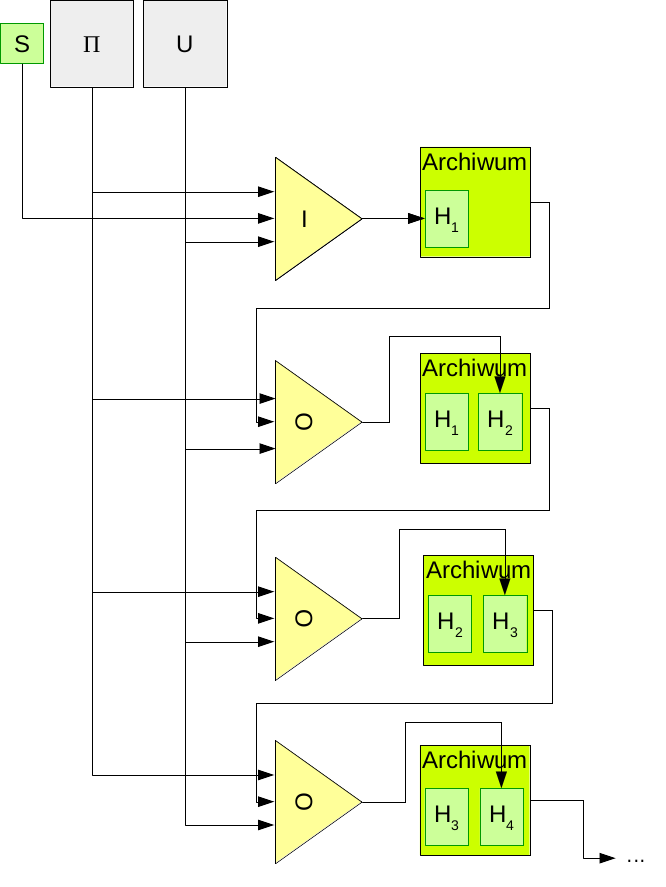
\includegraphics[scale=0.5]{img/ModelArchiwumFIFO2}\end{center}
\caption{Działanie heurystycznego algorytmu optymalizacyjnego z oknem archiwum wielkości równej dwukrotności osobników generowanych przez pojedynczą iterację. Zastosowano okno archiwum będące kolejką FIFO.}
\label{ModelArchiwumImg}
\end{figure}
\par{
I tak na przykład w opisanym w rozdziale \ref{DEvol_section} klasycznym algorytmie ewolucji różnicowej, mamy do czynienia z archiwum o rozmiarze równym wielkości populacji. Oznacza to, że do przeprowadzenia iteracji $N+1.$ algorytmu, oprócz $\Pi$ oraz $U$ potrzebujemy także wyniku $N.$ iteracji, ale już nie wyniku iteracji $N-1$. a tym bardziej całego archiwum $H$.
}
\par{
Tego rodzaju ograniczenia w wykorzystywaniu archiwum $H$ skłaniają do rozważań nad możliwością i stosownością wykorzystania informacji lub przesłanek ukrytych w nieużwanej części archiwum do poprawienia funkcjonowania algorytmu. Nie jest koncepcją nową [IGdzieŹródło] by parametryzować wykorzystywaną wielkość okna archiwum -- umożliwiając w ten sposób strojenie algorytmu oraz poprawianie jakości uzyskiwanych rezultatów. Pojawia się więc przypuszczenie, że także w przypadku ewolucji różnicowej powiększenie wykorzystywanego okna archiwum może umożliwiać uzyskiwanie lepszych jakościowo wyników optymalizacji.
}

\section{Algorytmy ewolucyjne}
\par{
Przykładem algorytmów heurystycznych stosowanych do rozwiązywania problemu optymalizacyjnego są algorytmy należące do grupy algorytmów ewolucyjnych (ang. \emph{Evolutionary Algorithms} -- AE) \cite{WykladyEvol,SpringerIntroToEvol}. Algorytmy te, wzorowane na ewolucji naturalnej operują pojęciami takimi jak osobnik, środowisko czy przystosowanie w celu adaptacyjnego przeszukiwania przestrzeni optymalizacyjnej.
}
\par{
Ogólna idea stojąca za algorytmami ewolucyjnymi, polega na opisaniu genotypu osobników, z których następnie można odczytać fenotyp (stanowiący punkt przestrzeni przeszukiwań) oceniany przez środowisko (funkcję optymalizowaną). Osobniki -- podobnie jak osobniki w naturze -- podlegają krzyżowaniu oraz niewielkim mutacjom, walcząc między sobą o zasoby naturalne. Zgodnie z teorią doboru naturalnego, osobniki gorzej dostosowane do środowiska są -- w szerokiej perspektywnie czasowej i przy odpowiednio dużej populacji -- wypierane przez te dostosowane lepiej [MS: MożeJakieśŹródłoNaDobórNaturalny? Darwin?].
}
\par{
/Note:Obrazek ze schematem EA?/
}
\par{
W związku z powyższą analogią w ramach algorytmów ewolucyjnych wyróżnia się następujące operatory:
\begin{description}
  \item[Krzyżowanie] -- to operator opisujący w jaki sposób na podstwie genotypu dwóch lub więcej osobników wytworzyć genotyp jednego lub więcej osobnika potomnego.
  \item[Mutacja] -- to operator wprowadzający genotypie wybranego osobnika losowe (nieznaczne) zabużenie.
  \item[Selekcja] -- to operator odpowiadający selekcji naturalnej, który oceniając osobniki na podstawie przystsowania ich fenotypu do środowiska odrzuca część znich preferując pozostawienie w populacji osobników lepiej dostosowanych.
  \item[Dobór do krzyżowania] -- to operator wybierający zestawy osobników podlegające krzyżowaniu. Operator ten opisuje znany z natury mechanizm preferencji (fenotypowej) organizmów przy rozmnażaniu.
  \item[Dobór do mutacji] -- to operator wybierający, które spośród osobników w populacji należy poddać mutacji. Odpowiada on zmiennemu w zależności od fenotypu organizmu prawdopodobieństwu wystąpienia u niego mutacji.
  \item[Inicjalizacja] -- to operator nieco oderwany od teorii ewolucji (gdyż ta nie opisuje powstawania pierwszych organizmów) opisujący sposób wygenerowania populacji początkowej spośród wszystkich możliwych genotypów.
  %%% dopasowanie do zakresu
\end{description}
}
\newpage
\par{
Ogólny schamat działania algorytmu ewolucyjnego opiera się o iteracyjną adaptację populacji aż do ustalonego warunku stopu, według następujących kroków:
\lstset{language=C}
\begin{lstlisting}[frame=single,mathescape]
P = Inicjalizacja(N)
while (!stop) {
	P $\cup$ Krzyzowanie(DoborDoKrzyzowania(P))
	P $\cup$ Mutacja(DoborDoMutacji(P))
	P = Selekcja(P)
}
\end{lstlisting}
}
\par{
W tym miejscu warto nadmienić, że choć w powyższym opisie algorytmów ewolucyjnych jest wprost mowa o podziale na genotyp i fenotyp, to na potrzeby zdefiniowanego problemu pojęcie fenotypu będzie wystarczające. Algorytmy opierające się o operacje na zakodowanym genotypie oderwanym od jego semantyki stanowią odrębną gałąź algorytmów ewolucyjnych i są nazywane algorytmami genetycznymi. Algorytmy te, ze względu na specyfikę swojego działania wymagają odpowiedniej reprezentacji danych i odpowiednio dobranych do reprezentacji operatorów. W przypadku rozważanego w pracy problemu optymalizacji, operowanie bezpośrednio na fenotypie ocenianym przez środowisko (a więc wektorach liczb rzeczywistych dla których wyznaczane są wartości funkcji optymalizowanej) ze względu na właściwości i możliwości samych liczb rzeczywistych wydaje się być w zupełności wystarczające. Zagadnienie podziału na genotyp i fenotyp będzie w dalszej części pracy zaniedbane.
}
\subsubsection{Eksploracja i Eksploatacja}
\par{
Ważnymi pojęciami opisującymi sposób w jaki osobniki w ramach algorytmów ewolucyjnych przszukują przestrzeń są pojęcia \textbf{eksporacji} i \textbf{eksploatacji}. Definiują one dwutorowe działanie grup osobników:
\begin{description}
  \item[Eksploracja] -- to proces poszukiwania nowych, przyciągających osobniki obszarów przestrzeni przeszukiwań charakteryzujących się niską wartością funkcji przystosowania. Pojęcie to opisuje proces poszukiwania w całej przestrzeni obszarów przyciągania wielu minimów lokalnych. 
  \item[Eksploatacja] -- to proces badania obszaru przestrzeni przeszukiwań charakteryzującego się niską średnią wartością funkcji przystosowania. Pojęcie to opisuje proces poszukiwania minimum lokalnego przez punkty zawierające się w jego obszarze przyciągania.
\end{description}
}
\par{
Uzyskanie właściwego balansu między tymi dwoma aspektami działania algorytmów ewolucyjnych jest kluczowe dla powodzenia algorytmu ewolucyjnego. Efekt sterowania siłą dwóch charakterystyk przeszukiwań otrzymuje się, przez odpowiednie definiowanie operatorów oraz ich parametrów. W szczególności, zadaniem operatora krzyżowania jest przede wszystkim prowadzenie populacji w kierunku ekspoalatacji, natomiast zadaniem mutacji jest generowanie punktów poza w danej chwili badanym obszarem przyciągania - a więc eksploracja przestrzeni przeszukiwań. Istosnym elementem regulującym tę równowagę jest także operator selekcji, której charakter znacząco wpływa na przeżywalność i siłę przyciągania osobników pionierów (wygenerowanych losowo, nielicznych punktów, w nowym, atrakcyjnym obszarze przyciągania).
}

\subsection{Ewolucja różnicowa}
\label{DEvol_section}
\par{
(Ogólny opis)
}
\par{
(Czym się różni od klasycznych algorytmów ewolucyjnych)
}
\par{
(Zalety i wady w kontekście problemu optymalizacji)
}
\par{
(Parametry)
}
\par{
(Wyniki w kontekście innych metod)
}
\par{
(Idea punktu środkowego)
}
\par{
(Metody uwzględniania ograniczeń)
}

\subsubsection{Podejście do archiwum}
\par{(Odniesienia w literaturze)}
\par{(Dotychczasowe wnioski)}

\section{Metodyka badań (opisywać tak szeroko?)}
\subsection{Modelowanie statystyczne}
\par{
(Czemu służy, dlaczego potrzebne do tych badań)
}
\subsection{Testy statystyczne}
\par{
(Ogólna koncepcja, p-value)
}
\subsection{Testy parametryczne}
\par{
(Co to jest i kiedy się stosuje)
}
\subsubsection{Test T-studenta}
\par{
(Jak działa, ZAŁOŻENIA)
}
\par{
(Wady zalety).
}

\subsection{Testy nieparametryczne}
\par{
(Co to jest i kiedy się stosuje)
}
\subsubsection{Test wilcoxona}
\par{
(Opis, działanie, ZAŁOŻENIA)
}
\par{
(Wady zalety)
}
\section{Benchmarki blackboxowe}
\par{
(Czemu służą)
}
\par{
(Dlaczego są dobrym odniesieniem)
}

\subsection{CEC}
\par{
(Opis benchmarka, funkcje testowe)
}
\par{
(Implementacja w R)
}

\chapter{Algorytm DEArch}

\par{

}
\section{Podejścia do wykorzystania archiwum}
\subsection{Wybór punktów do archiwum}
\subsection{Podejście do normalizacji}

Podstawowym celem modyfikacji algorytmu ewolucji różnicowej, było ograniczenie ilości osobników w pokoleniu bez utraty ilości możliwych do wygenerowania wektorów różnicowych. Mając to założenie na względzie rozpatrzono kilka wariantów archiwum punktów.
\section{Kompletna definicja algorytmu}

\chapter{Badania}
\section{Cel}
\section{Plan eksperymentów}
\section{Dobór parametrów}
\section{Zbierane rezulataty}
\subsection{Środek ciężkości populacji (DE/mid)}
\section{Sposób analizy}

\section{Wyniki (w załączniku?)}
\section{Analiza wyników (wnioski)}

\chapter{Podsumowanie}


\bibliographystyle{plplain}
\nocite{*}
\bibliography{bibliography}

\end{document}
